%%%%%%%%%%%%%%%%%%%%%%%%%%%%%%%%%%%%%%%%%
% Beamer Presentation
% LaTeX Template
% Version 1.0 (10/11/12)
%
% This template has been downloaded from:
% http://www.LaTeXTemplates.com
%
% License:
% CC BY-NC-SA 3.0 (http://creativecommons.org/licenses/by-nc-sa/3.0/)
%
%%%%%%%%%%%%%%%%%%%%%%%%%%%%%%%%%%%%%%%%%

%----------------------------------------------------------------------------------------
%   PACKAGES AND THEMES
%----------------------------------------------------------------------------------------

\documentclass{beamer}
%encoding
%--------------------------------------
\usepackage[utf8]{inputenc}
\usepackage[T1]{fontenc}
%--------------------------------------
 
%Portuguese-specific commands
%--------------------------------------
\usepackage[portuguese]{babel}
%--------------------------------------

\mode<presentation> {

% The Beamer class comes with a number of default slide themes
% which change the colors and layouts of slides. Below this is a list
% of all the themes, uncomment each in turn to see what they look like.

%\usetheme{default}
%\usetheme{AnnArbor}
%\usetheme{Antibes}
%\usetheme{Bergen}
%\usetheme{Berkeley}
%\usetheme{Berlin}
%\usetheme{Boadilla}
%\usetheme{CambridgeUS}
%\usetheme{Copenhagen}
%\usetheme{Darmstadt}
%\usetheme{Dresden}
%\usetheme{Frankfurt}
%\usetheme{Goettingen}
%\usetheme{Hannover}
%\usetheme{Ilmenau}
%\usetheme{JuanLesPins}
%\usetheme{Luebeck}
\usetheme{Madrid}
%\usetheme{Malmoe}
%\usetheme{Marburg}
%\usetheme{Montpellier}
%\usetheme{PaloAlto}
%\usetheme{Pittsburgh}
%\usetheme{Rochester}
%\usetheme{Singapore}
%\usetheme{Szeged}
%\usetheme{Warsaw}

% As well as themes, the Beamer class has a number of color themes
% for any slide theme. Uncomment each of these in turn to see how it
% changes the colors of your current slide theme.

%\usecolortheme{albatross}
%\usecolortheme{beaver}
%\usecolortheme{beetle}
%\usecolortheme{crane}
%\usecolortheme{dolphin}
%\usecolortheme{dove}
%\usecolortheme{fly}
%\usecolortheme{lily}
%\usecolortheme{orchid}
%\usecolortheme{rose}
%\usecolortheme{seagull}
%\usecolortheme{seahorse}
%\usecolortheme{whale}
%\usecolortheme{wolverine}

%\setbeamertemplate{footline} % To remove the footer line in all slides uncomment this line
%\setbeamertemplate{footline}[page number] % To replace the footer line in all slides with a simple slide count uncomment this line

%\setbeamertemplate{navigation symbols}{} % To remove the navigation symbols from the bottom of all slides uncomment this line
}

\usepackage{graphicx} % Allows including images
\usepackage{booktabs} % Allows the use of \toprule, \midrule and \bottomrule in tables

%----------------------------------------------------------------------------------------
%   TITLE PAGE
%----------------------------------------------------------------------------------------

\title[Programação Funcional]{Programação Funcional } % The short title appears at the bottom of every slide, the full title is only on the title page

\author{Emylle,Jamile,Filipe,Gabriel,Daniel,Wyllyan} % Your name
\institute[UCLA] % Your institution as it will appear on the bottom of every slide, may be shorthand to save space
{
IFAL - Instituto Federal de Alagoas     \\
\medskip
\textit{} % Your email address
}
\date{\today} % Date, can be changed to a custom date

\begin{document}

\begin{frame}
\titlepage % Print the title page as the first slide
\end{frame}

\begin{frame}
\frametitle{Introdução Básica} % Table of contents slide, comment this block out to remove it
\tableofcontents % Throughout your presentation, if you choose to use \section{} and \subsection{} commands, these will automatically be printed on this slide as an overview of your presentation
\end{frame}

%----------------------------------------------------------------------------------------
%   PRESENTATION SLIDES
%----------------------------------------------------------------------------------------

%------------------------------------------------
\section{Programação funcional, é um paradigma de programação, uma maneira de se programar, que utiliza de um código composto de múltiplas funções que se compõem para resolver um problema. Por exemplo, se eu tenho um dado de entrada e preciso transformá-lo em um dado de saída. Eu vou juntar as lógicas de transformações do meu código em funções, e usá-las no melhor momento para transformar este meu dado. } % Sections can be created in order to organize your presentation into discrete blocks, all sections and subsections are automatically printed in the table of contents as an overview of the talk
%------------------------------------------------

\subsection{ Evita repetições \newline Código limpo  
\newline Facilidade de leitura 
\newline Mutações no código mais agilizadas
} % A subsection can be created just before a set of slides with a common theme to further break down your presentation into chunks

\begin{frame}
\frametitle{Introdução Básica}
O que difere a programação funcional da programação imperativa, por exemplo, é a utilização de métodos que facilitam na minimização do código. Entretanto, sua curva de aprendizado é maior, visto que estamos lidando com um novo conceito, que dificilmente é ensinado “logo de cara” nas instituições de ensino. \\~\\
Vejamos um exemplo de comparação:

\end{frame}


%------------------------------------------------

\begin{frame}
\frametitle{Introdução Básica}
\begin{figure}[!ht]
    \centering
    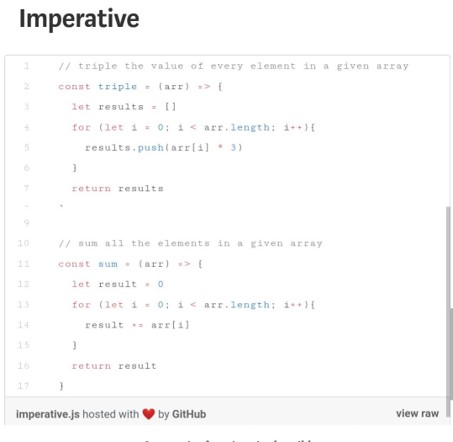
\includegraphics[width=.5\columnwidth]{Imagens/Imagem1.jpg}
    \caption{Imperative}
    \label{fig:my_label}
\end{figure}

\end{frame}


\begin{frame}
\frametitle{Introdução Básica}
\begin{figure}[!ht]
    \centering
    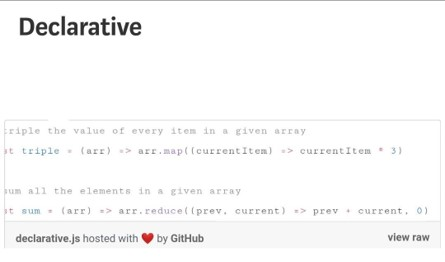
\includegraphics[width=.8\columnwidth]{Imagens/Imagem2.jpg}
    \caption{Declarative}
    \label{fig:my_label}
\end{figure}

\end{frame}





\begin{frame}
\frametitle{Introdução Básica}
É fácil identificar a diferença. Pôde se resumir, através de dois métodos as duas funções realizadas na imperativa. .map() é um método acessível a partir de qualquer array no JS. O método .map () cria um novo array com os resultados da chamada de uma função fornecida em todos os elementos da matriz de chamada. O método.reduce() adiciona na função um acumulador a cada elemento da lista (array) da esquerda para a direita até que seja reduzido a um único valor. 
Com isso o código fica sucinto e fácil de ser compreendido. 
\newline Veremos agora alguns conceitos desse paradigma. 


\end{frame}

%------------------------------------------------

\begin{frame}
\frametitle{Imutabilidade}
Uma vez que uma variável é criada, seu valor nunca será alterado.
\end{frame}

%------------------------------------------------
\begin{frame}
\frametitle{Abstração e Modularização}
Fundamental para a Modularização
\newline Seleção que deve ser representado
\newline Possibilita a divisão do trabalho em níveis
\newline Foco na Distinção entre:
\centerline{O que uma parte do programa faz}
\centerline{Como isso é implementado}
\newline \newline Abstrações de Processos
\newline \newline Abstração de Dados

\end{frame}
%------------------------------------------------
%------------------------------------------------
%------------------------------------------------
\begin{frame}
\frametitle{Funções}
Não é a toa que programação funcional é a programação “orientada a funções”. O conceito de função matemática permeia este paradigma.
\newline Funções Puras: Bem, o conceito de funções puras tem tudo a ver com a não existência de efeitos colaterais. Funções puras são funções que não modificam o escopo ao redor delas.
\newline
\newline Uma função pura: Recebe ao menos um parâmetro e trabalha com ele.
Ela retorna alguma coisa. É interessante que uma função, como nos ensinam, via de regra, é uma sequencia de procedimentos a serem executados. Até ai, tudo bem, porem, em programação funcional uma função sempre deve retornar um valor. 
\newline Por que? Encadeamento de operações. 

\end{frame}


\begin{frame}
\frametitle{Funções}
\begin{figure}
    \centering
    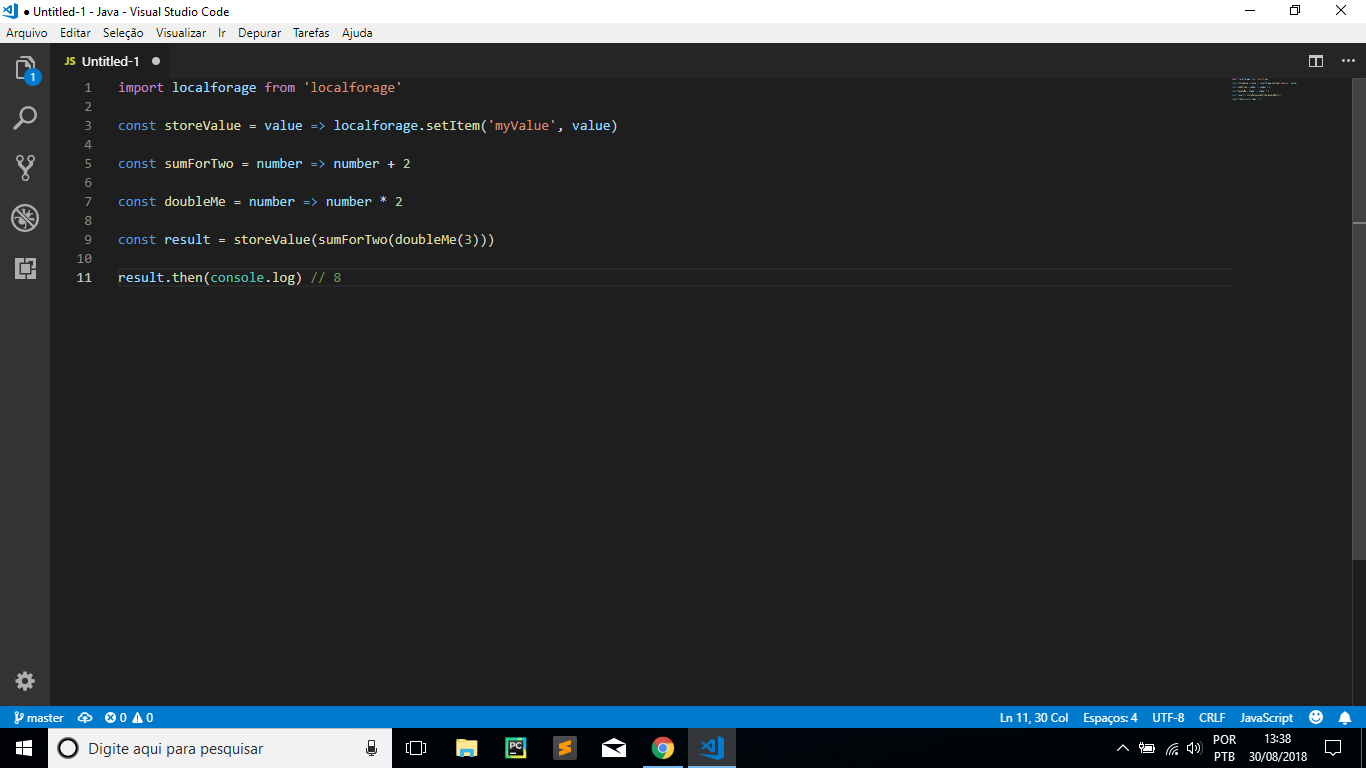
\includegraphics[width=.9\columnwidth]{Imagens/Imagem3.png}
    \caption{Função Pura}
    \label{fig:my_label}
\end{figure}

\end{frame}


\begin{frame}
\frametitle{Funções}
Funções de primeira classe: Quando uma linguagem possui first-class function, significa que funções podem ser usadas como valores, sendo passadas como parâmetros e recebidas como resultados. Em suma, uma first-class function é uma função que representa um valor no código, pode ser um array, um objeto…
\newline 
\newline Funções de primeira ordem: 
Uma linguagem que possui high-order functions, é aquela em que suas funções podem ter outras funções como parâmetros e retornar ou não, elas como resultado.
\end{frame}

%------------------------------------------------


%------------------------------------------------

\begin{frame}
\frametitle{Referências Bibliográficas}
\footnotesize{
\begin{thebibliography}{99} % Beamer does not support BibTeX so references must be inserted manually as below
\newblock https://hackernoon.com/javascript-and-functional-programming-an-introduction-286aa625e26d
\newblock {“Javascript and Functional Programming: An Introduction” }
\newblock https://medium.com/trainingcenter/programação-funcional-para-iniciantes-9e2beddb5b3
\newblock {“Programação funcional para iniciantes” @EmanuelGDev  }

\end{thebibliography}



}
\end{frame}

%------------------------------------------------

\begin{frame}
\Huge{\centerline{The End}}
\Huge{\centerline{Fim}}
\Huge{\centerline{Quem gostou bate palmas}}
\Huge{\centerline{quem não gostou paciência}}
\end{frame}

%----------------------------------------------------------------------------------------

\end{document}